\section{Analysis}
\label{chapter3}

\begin{figure}[H]
	\centering
	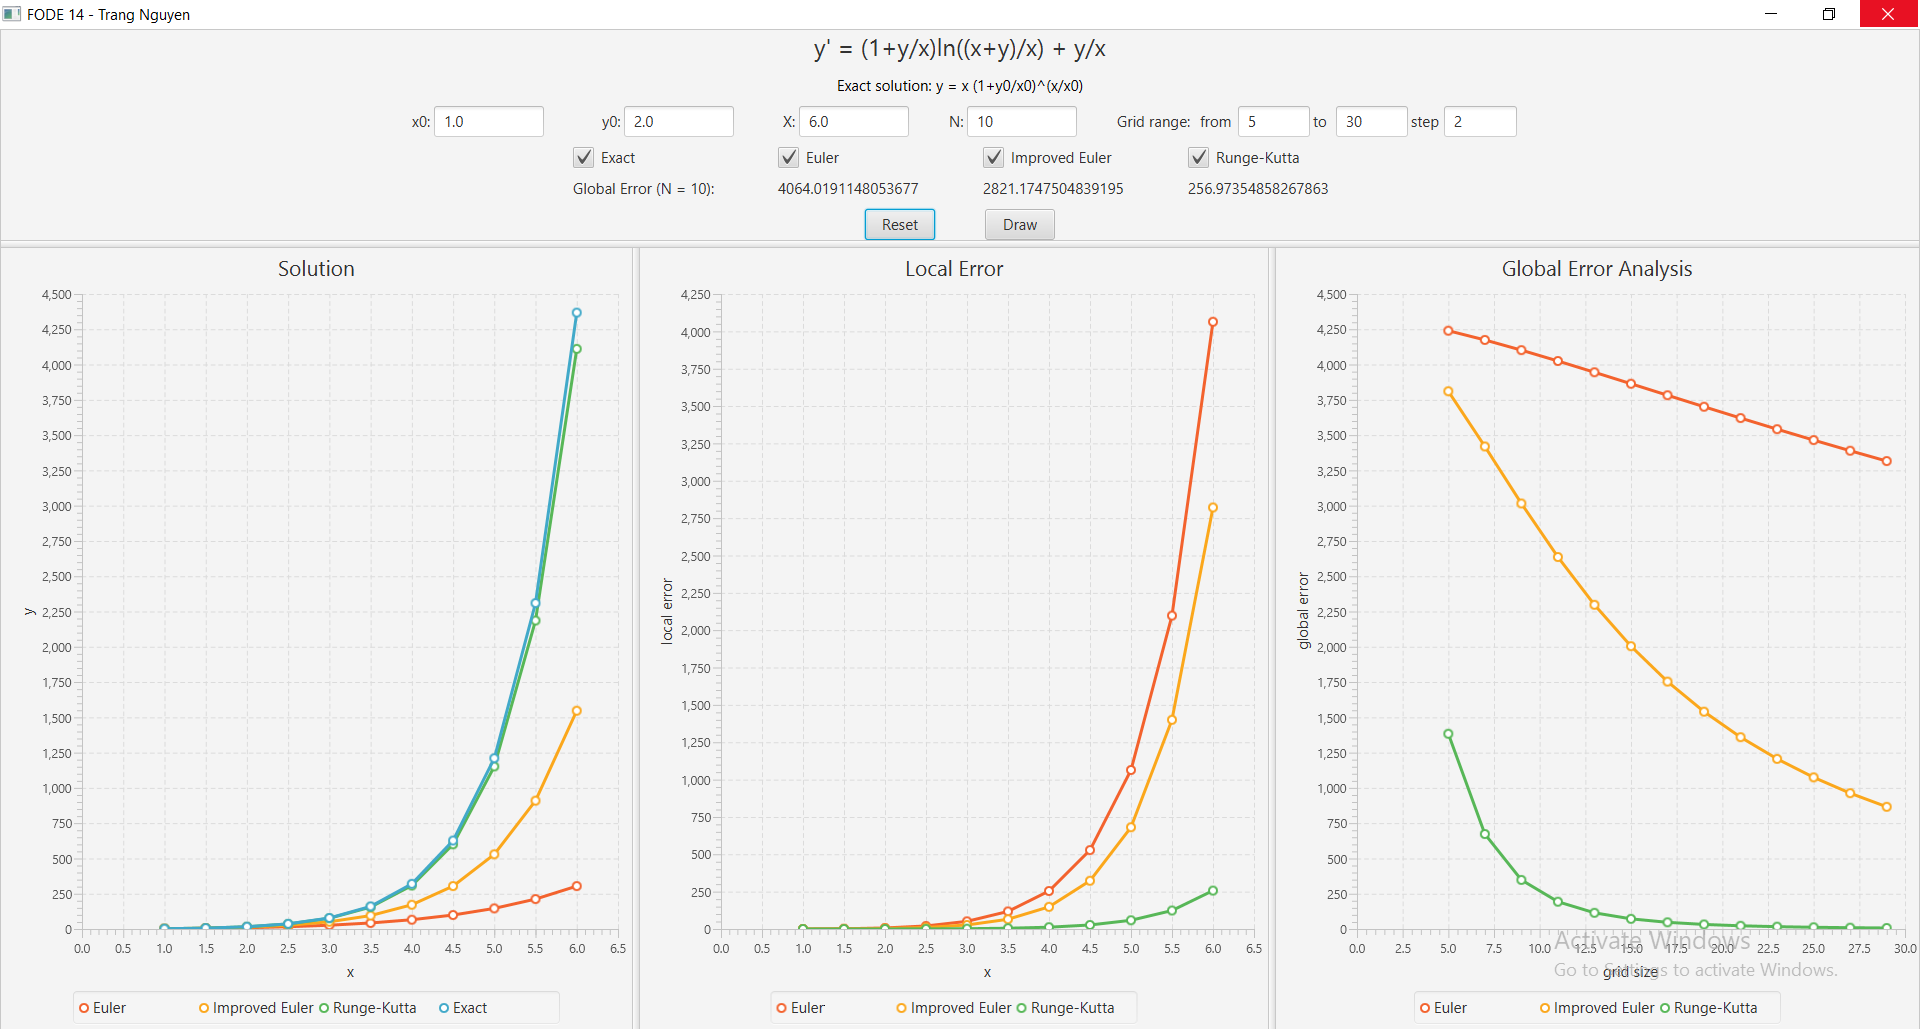
\includegraphics[width=\linewidth]{image/full.png}
	\caption{Analysis with $x_0=0.1$, $y_0=2$, $X=6.0$, $N=10$, grid range = $(5,30,2)$}
	\label{fig:applicationscreenshot}
\end{figure}

Analyzing using the software, we can infer that:
\begin{itemize}  
\item Runge-Kutta method has the highest performance (closest to exact solution, lowest local and global errors). Following is Improved Euler, and Euler method.
\item For $x_0=0.1$, $y_0=2$, $X=6.0$, from $N=20$, increasing $N$ does not significantly affect accuracy of Runge-Kutta method. This number for improved Euler method is around 150, and for Euler method is around 2000.
\end{itemize}